\documentclass[11pt,a4paper]{article}
\usepackage[utf8]{inputenc}
\usepackage{amsmath, mathtools}
\usepackage{amsfonts, dsfont}
\usepackage{amssymb}
\usepackage{graphicx}
\usepackage{empheq}
\usepackage{bm}
\usepackage[round, sort]{natbib}
\usepackage{tikz}
\usepackage{mathtools}  
%\mathtoolsset{showonlyrefs}  
\usetikzlibrary{shapes,backgrounds,arrows,automata,snakes,shadows,positioning, mindmap}

%%%%% Commands
\newcommand{\argmin}{\arg\!\min}
\newcommand{\argmax}{\arg\!\max}
\newcommand*\widefbox[1]{\fbox{\hspace{3em}#1\hspace{3em}}}
\newcommand*\lesswidefbox[1]{\fbox{\hspace{2em}#1\hspace{2em}}}
\newcommand{\entr}{\mathcal{H}}
\newcommand{\betabf}{\boldsymbol{\beta}}
\newcommand{\thetabf}{\boldsymbol{\theta}}
\newcommand{\mubf}{\boldsymbol{\mu}}
\newcommand{\Omegabf}{\boldsymbol{\Omega}}
\newcommand{\Sigmabf}{\boldsymbol{\Sigma}}
\newcommand{\zerobf}{\boldsymbol{0}}
\newcommand{\Xbf}{\boldsymbol{X}}
\newcommand{\xbf}{\boldsymbol{x}}
\newcommand{\Ybf}{\boldsymbol{Y}}
\newcommand{\Zbf}{\boldsymbol{Z}}
\newcommand{\Sbf}{\boldsymbol{S}}
\newcommand{\mbf}{\boldsymbol{m}}
\newcommand\Ncal{\mathcal{N}}
\newcommand\Pcal{\mathcal{P}}
\newcommand\Tcal{\mathcal{T}} 
\newcommand{\Esp}{\mathds{E}}
\newcommand{\bound}{\mathcal{J}}
 
 %%%%%%% TIKZ
 \newcommand{\edgeunit}{1.5}
\providecommand\given{} % is redefined in \Set
\newcommand\SetSymbol[1][]{\nonscript\:#1\vert\nonscript\:}
%\usepackage[mathcal]{eucal}
\usepackage[left=2cm,right=2cm,top=2cm,bottom=2cm]{geometry}
\tikzset{%
    observed/.style={%
    scale=0.9,rectangle,draw=white,transform shape,fill=white,font=\Large}
}
\tikzset{%
    basic/.style={%
    scale=0.9,circle,draw=black,transform shape,fill=white,font=\small}
}


\setlength\parindent{0pt}
 \setcounter{tocdepth}{2}
\title{Reconstruction of a missing actor from count data using network inference}

\begin{document}

\maketitle
\vspace{3cm}
\tableofcontents
\newpage
Previously:
$$ p(\Ybf,\Zbf,T) = p(T)p(\Zbf|T)p(\Ybf|\Zbf)$$
$$ \Esp(\log p(\Ybf,\Zbf,T)|\Ybf) \approx \sum_{1 \leq j < k \leq p} P_{jk} \log\left(\beta_{jk} \hat{\psi}_{jk}\right) - \log B + cst$$

Now adding a hidden layer of unobserved data, indexed by H:

$$ p(\Ybf,\Zbf_O,\Zbf_H,T)$$
\section{PLNmissing peculiarities:}

\subsection{Model}

$$\left\{\begin{array}{rl}
T & \sim\prod_{jk \in T} \beta_{jk}/B \\\\
\Zbf|T& \sim\mathcal{N}(0,\Sigma_T)\\\\
\Ybf|\Zbf&\sim\mathcal{P}( \exp( \Xbf\theta^\intercal + \Zbf) )
\end{array} \right.$$

\paragraph{Dimensions:}
The model is build on matrices $\Ybf$ and $\Zbf$ with the following dimensions:\\
$\Ybf$: $n\times p$\\
$\Zbf_O$: $n\times p$\\
$\Zbf_H$: $n\times r$


\paragraph{Underlying dependencies:} This diagram is the graphical model behind the model, it describes the variables direct denpendencies and how data is simulated. Here, a tree $T$ is first drawn, which controls the dependency structure of parameters $\Zbf = (\Zbf_O,\Zbf_H)$. Count data $\Ybf$ is drawn from a distribution depending only on observed parameters $\Zbf_O$.
\begin{center}
	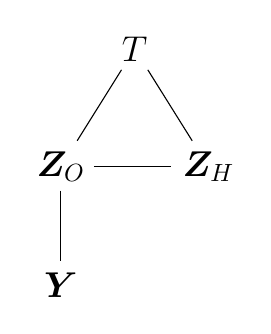
\begin{tikzpicture}	
      \tikzstyle{every edge}=[-,>=stealth',shorten >=1pt,auto,thin,draw]
		\node[observed] (A1) at (0.625*\edgeunit, 2*\edgeunit) {$T$};
		\node[observed] (A2) at (0*\edgeunit, 1*\edgeunit) {$\Zbf_O$};
		\node[observed] (A3) at (1.25*\edgeunit, 1*\edgeunit) {$\Zbf_H$};
		\node[observed] (A4) at (0*\edgeunit, 0*\edgeunit) {$\Ybf$};
		\path (A1) edge [] (A2)
        (A1) edge [] (A3)
        (A2) edge [] (A3)
        (A2) edge [] (A4);
	\end{tikzpicture}
\end{center}

\subsection{Distributions}
\label{distrib}
\paragraph{Marginals}
The complete vector of underlying parameters $Z$ follows a mixture of Gaussian laws on the space of all existing spanning trees.
\begin{align*}
(\Zbf_O,\Zbf_H) &\sim \sum_{T \in \mathcal{T}} p(T) \mathcal{N}(0,\Sigma_T) \\
\end{align*}

\paragraph{Conditional on T:}
Conditionally on the dependency structure $T$, $\Zbf$ is a centered Gaussian variable, with covariance matrix $\Sigma_T$ defined by block:
\[
 \Sigma=
  \left( {\begin{array}{cc}
  \Sigma_{TO} &  \Sigma_{TOH}\\\\
  \Sigma_{THO} & \Sigma_{TH}
  \end{array} } \right) =
   \left( {\begin{array}{cc}
  \Omega_{TO} &  \Omega_{TOH}\\\\
  \Omega_{THO} & \Omega_{TH}
  \end{array} } \right)^{-1}
  \]\\
This results in the following distributions:
\begin{align*}
(\Zbf_O,\Zbf_H)|T & \sim\mathcal{N}(0,\Sigma_T)\\
\Zbf_O|T & \sim\mathcal{N}(0,\Omega_{Tm}^{-1})\\
\end{align*}
With $ \Omega_{Tm} =\Sigma_{TO}^{-1} =  \Omega_{TO} - \Omega_{TOH}\Omega_{TH}^{-1}\Omega_{THO}$. This comes from the Schur's complement which is recalled in appendix.\\

A result from Lauritzen states that Gaussian precision matrices which are faithful to different trees will only differ in the position of their zero entries, meaning that any trees sharing  an edge will also share the same value in their precision matrix. Let's define $\Omega$ such as $$\forall T_a \in \{T \in\mathcal{T} / kl \in T \}, \Omega_{T_a}[k,l] =  \Omega [k,l].$$ Let's also define $I_T$ the binary matrix with diagonal one indicating the  edges presence in tree $T$ : $I_T=(\mathds{1}_{kl \in T} + \mathds{1}_{k=l})_{kl}$. Then we can write :
$$\forall T\in \mathcal{T}, \;\;\; \Omega_T = I_T \odot \Omega $$

For identifiability reasons, two hidden nodes cannot be linked with each. The $H$ bloc of $\Omega_T$ should thus be diagonal , and we get: 
\[
 \Omega_T=
  \left( {\begin{array}{cc}
 (I_T \odot \Omega)_O &  (I_T \odot \Omega)_{OH}\\\\
 (I_T \odot \Omega)_{HO} &   \Omega_H 
  \end{array} } \right) \]\\
  
  Note that the diagonal of $\Omega_T$ do not depend on $T$.
  
\paragraph{Conditional on observed data:\\}


As $\Zbf_O$ decouples $\Zbf_H$ and $\Ybf$, we will never need $\Zbf_H|\Ybf$:
$$ p(\Zbf|\Ybf) = p(\Zbf_O,\Zbf_H | \Ybf) = p(\Zbf_H|\Zbf_O) \: p(Z_O|\Ybf) $$




 In a precision matrix of a multivariate Gaussian, the conditional bloc is the marginal bloc:  $\Omega_{TH|O}^{-1} = \Sigma_{TH} -\Sigma_{THO}\Sigma_{TO}^{-1}\Sigma_{TOH} = \Omega_{TH}^{-1} =\Omega_{H}^{-1}$. Therefore the conditional distribution of the unobserved latent vectors given the latent observed ones is as follows: $$\Zbf_H|\Zbf_O,T \sim \mathcal{N}(\mu_{H|O,T}, \Omega_{H}^{-1})$$ 

  Let's $\Zbf_{Oi}$ denote a realization of $\mathcal{N}(0,\Sigma_{TO}) $. Then $\displaystyle  \mu_{H|Oi,T} = \Sigma_{THO}\Sigma_{TO}^{-1}(\Zbf_{Oi}-\underbrace{\mu_{\Zbf_Oi|T}}_{0}) 
 = -\Omega_{TH}^{-1}\Omega_{THO} \: \Zbf_{Oi}
$ 


\section{Variational EM inference}
\subsection{Approximation of the likelihood}
\paragraph{Joint likelihood:}
The graphical model gives the following writing of the joint likelihood:
\begin{align*}
p(\Ybf,Z,T)& = p(T) \: p(Z|T) \: p(\Ybf|Z) \\
&= p(T)\: p(Z_O,Z_H|T) \: p(\Ybf|Z_O,Z_H) \\
&= p(T) \: p(Z_O|T) \: p(Z_H | Z_O,T)  \: p(\Ybf|Z_O)
\end{align*} 


\paragraph{Variational approximation:}

Here $p(T,\Zbf \mid \Ybf)$ is untractable. We adopt a variational approximation aiming to maximise a lower bound of the log-likelihood of observed data $\log p(\Ybf)$, namely  
\begin{align*}
    \mathcal{J}(\Ybf; g,h)
    & = \log p(\Ybf) - KL\left[q(T,\Zbf) \middle\vert\middle\vert\ p(T,\Zbf \mid \Ybf)\right]
\end{align*}
Where KL is the Küllback-Leibler divergence. The approximation we adopt relies on factorizing $q$ in the product of two distributions $h$ and $g$ relating respectively to $\Zbf$  and $T$: 
$$p(T,Z | \Ybf) \approx  q(Z,T) = g(T)h(Z).$$

 A consequence of this hypothesis is the contributions of   $\Esp_h[\log p(\Zbf\mid T)]$ and $\log p(T)$ --~only terms involving $T$ in the lower bound~-- writing as sums on the edges. As distribution   $g$ minimizes the KL divergence, it has to factorizes on the edges as well and hence:
$ g(T) = \left(\prod_{kl} \widetilde{\beta}_{kl} \right) / \widetilde{B}$. \\
 
Moreover, it follows from the independence of the samples that $h$ is a product law: $ h(\Zbf) = \prod_i h_i(\Zbf_i)$.
Our variational approximation consists in assuming that each of its components is a multivariate Gaussian: $h(\Zbf_i) = \Ncal(\Zbf_i; \mbf_i, \Sbf_i)$, where $\Sbf_i$ is diagonal. More precisely:  $ h(Z_i) =  \mathcal{N}(m_i,S_i)$ , where $S_i$ is diagonal with diagonal $(s_{i1}^2, ... , s_{i(p+r)}^2)$, meaning that $\Zbf_H$ and $\Zbf_O$ are independent under distribution $h$. Marginals are written $h_O$  and  $h_H$. $S=\sum_i S_i$  and $ M =  [m_i]_{1 \leq i \leq (p+r)}$ (so $\Esp_h[Z_{\cdot k}^\intercal Z_{\cdot k}] = \sum_i s_{ik} + m_{\cdot k}^\intercal m_{\cdot k}$). $S$ is also diagonal and its H and O blocs are denoted $S_H$ and $S_O$. In the following, the $n\times p $ and $n\times r $ matrices $M_O$ and  $M_H$ compile all vectors of means $\mbf_i$ corresponding respectively to observed and hidden latent vectors ; $M_O$ and  $M_H$ are gathered in matrix $M= (M_O | M_H)$.

 
%In the following we use the scalar product on the matrix space defined with the trace operator as: 
%$$  Tr(A^\intercal B) = <A,B> .$$
\paragraph{Lower bound:}
Starting with the two hidden layers of our model, the lower bound writes:
\begin{align*}
\mathcal{J}(\Ybf; g,h)&=\log p(\Ybf) - KL\left[g(T) h(\Zbf) \middle\vert\middle\vert\ p(T,\Zbf | \Ybf)\right]\\
&= \log p(\Ybf) - \Esp_{gh}[\log( g(T) h(\Zbf)) - \log p(\Zbf,T\mid \Ybf) ]\\
&= \log p(\Ybf) - \Esp_{gh}[\log g(T) + \log h(\Zbf) ] + \Esp_{gh}[\log p(\Ybf,\Zbf,T)] - \Esp_{gh}[\log p(\Ybf)]\\
&= \Esp_{gh} [\log p(\Ybf,\Zbf,T)] + \entr[g(T)] + \entr[h(\Zbf)]
\end{align*}

\begin{equation}
\label{firstJ}
 \boxed{\mathcal{J}(\Ybf; g,h) = \Esp_{gh} [\log (p_\beta(T)p_{\Omega}(\Zbf\mid T)p_\theta(\Ybf\mid \Zbf))] + \entr[g_{\widetilde{\beta}}(T)] + \entr[h_{M,S}(\Zbf)]}
\end{equation}
Thus the model's parameters are $\Phi = (\beta, \Omega, \theta, \widetilde{\beta},M,S)$.
\subsection{Optimizing in $\theta$ and $h(\Zbf_O)$:}
\citet{CMR18} compute the lower bound of a VEM for the original PLN, which we write $\mathcal{J}_{PLN}$,  in the R package \textit{PLNmodels}. It is possible to use $\mathcal{J}_{PLN}$ in our computation as well, the following shows how.

Let's first separate observed and unobserved latent variables:
\begin{align*}
\mathcal{J}(\Ybf; g,h)&= \Esp_{gh}[\log p(T)  p(\Zbf_H| \Zbf_O,T) p(\Zbf_O|T)p(\Ybf|\Zbf_O)] + \entr[g(T)] +\entr[h(\Zbf_H,\Zbf_O)]
\end{align*}

 We develop the entropy of the complete $\Zbf$ vector, to make the entropy of $\Zbf_O$ appear. $\Zbf_O$ and $\Zbf_H$ being independant under the $h$ distribution, we have:
\begin{align*}
\entr[h(\Zbf_H,\Zbf_O)] &= -\Esp_h[\log h(\Zbf_H,\Zbf_O)] =-\Esp_h[\log h(\Zbf_H)] - \Esp_h[\log \Zbf_O)]\\
&=\entr[h(\Zbf_O)] +\entr[h(\Zbf_H)]
\end{align*}

Now using the hypothesis of independence of $g$ and $h$, we can obtain quantities with separate dependencies:
\begin{align}
\mathcal{J}(\Ybf; g,h)&=  \Esp_{gh}[\log p(\Zbf_O | T)] +\Esp_h[\log p(\Ybf|\Zbf_O)]+\entr[h(\Zbf_O)]  \label{PLNlike}\\
& \;\; + \Esp_{gh}[\log p(\Zbf_H | \Zbf_O,T) ]+\Esp_g[\log p(T)] +\entr[g(T)]+\entr[h(\Zbf_H)] \label{new}
\end{align}

Let's then detail the first term of the lower bound:
\begin{align*}
\Esp_{gh}[\log p(\Zbf_O|T)] &=  \Esp_{gh} \left[\frac{n}{2} \log |\Omega_{Tm}| - \frac{1}{2} \sum_i \Zbf_{Oi}\Omega_{Tm} \Zbf_{Oi}^\intercal  \right]\\
&= \frac{n}{2} \Esp_g [\log |\Omega_{Tm}|] - \frac{1}{2} \Esp_{gh}\left[Tr\left( \Zbf_O^\intercal \Zbf_O \Omega_{Tm}\right)\right].
\end{align*}

The expectation in $gh$ is again separable thanks to the independence hypothesis. As the trace is a linear operation we obtain:
\begin{align*}
\Esp_{gh}[\log p(\Zbf_O|T)] &=\frac{n}{2} \Esp_g [\log |\Omega_{Tm}|] - \frac{1}{2}  Tr\left(\Esp_h [\Zbf_O^\intercal \Zbf_O ]\; \Esp_g[\Omega_{Tm}]\right) 
\end{align*}
$\Esp_g [\Omega_{Tm}]$ is a $p\times p$ matrix of expected inverse covariance over the whole spanning-tree space. Introducing the quantity  $\log |\Esp_g [\Omega_{Tm}]| $ in part (\ref{PLNlike}) of $\mathcal{J}(\Ybf; g,h)$:
\begin{align*}
&\Esp_{gh}[\log p(\Zbf_O | T)] +\Esp_h[\log p(\Ybf|\Zbf_O)]+ \entr[h(\Zbf_O)]\\
& = \frac{n}{2} \log |\Esp_g [\Omega_{Tm}]| - \frac{1}{2}Tr\left(\Esp_h [\Zbf_O^\intercal \Zbf_O ]\; \Esp_g[\Omega_{Tm}]\right)+ \Esp_{h}[\log p(\Ybf|\Zbf_O)] + \entr[h(\Zbf_O)]\\
& \;\;\;+  \frac{n}{2}\left( \Esp_g[\log|\Omega_{Tm}|] - \log|\Esp_g [\Omega_{Tm}]|\right)
\end{align*}
%The second line is a negative quantity, because the log determinent is a concave function. Jensen's inequality gives:
%$$\log |\Esp_g[\Omega_{Tm}]| \geq \Esp_g [\log |\Omega_{Tm}|]$$
%$$ \Esp[Z_jZ_k] = -\partial_{\omega_{jk}}( \log |\Omega_{TO}| )$$
%Therefore,
Assuming $\Esp_g [\Omega_{Tm}]$ is an inverse variance covariance matrix for $\Zbf_O$, the lower bound $\mathcal{J}_{PLN}$ appears:
 $$\Esp_{gh}[\log p(\Zbf_O | T)] +\Esp_h[\log p(\Ybf|\Zbf_O)]+ \entr[h(\Zbf_O)] = \mathcal{J}_{PLN} - \frac{n}{2}\left( \Esp_g[\log|\Omega_{Tm}|] - \log|\Esp_g [\Omega_{Tm}]|\right)$$
 
As the last term do not depend either on $\theta$ or $h(\Zbf_O)$, we finally obtain that
 $$ \argmax_{\theta, h(\Zbf_O)} \big\{\Esp_{gh}[\log p(\Zbf_O | T)] +\Esp_h[\log p(\Ybf|\Zbf_O)]+ \entr[h(\Zbf_O)]\big\} = \argmax_{\theta, h(\Zbf_O)} \big\{ \mathcal{J}_{PLN} \big\}.$$

The VE step of PLNmodels VEM algorithm maximizes $\mathcal{J}_{PLN}$ and gives estimates of $\Zbf_O$ moments of order 1 and 2, so we have easy access to estimates $\widetilde{M}_O$ and $\widetilde{S}_O$. As there are still some dependence in $h(\Zbf_O)$ in part (\ref{new}) of $\mathcal{J}(\Ybf; g,h)$, using $\argmax_{\theta, h(\Zbf_O)} \big\{ \mathcal{J}_{PLN} \big\}$ maximizes  $\mathcal{J}(\Ybf;g,h)$ in $\theta$, and only partly in $h(\Zbf_O)$. Therefore   the proposed solution is sub-optimal. \\

After maximizing part (\ref{PLNlike}) of $\mathcal{J}(\Ybf; g,h)$ in $h_O$, this density is considered constant and written $h_O^*$.  We can then write the partly optimized  lower bound as follows:
\begin{align*}
\mathcal{J}_{h_O^*}(\Ybf; g,h)&= \Esp_{h_O^*}[\log p(\Ybf \mid \Zbf_O)] - \Esp_{h_O^*}[\log h(\Zbf)] + \Esp_{gh}[\log p(\Zbf \mid T)] + \Esp_g \big[\log p(T) - \log g(T) \big]
\end{align*}

 Note that $\Esp_{h_O^*}[\log h(\Zbf)]$ is now completely optimized in $h$, as it is a Gaussian entropy therefore only depending on its variance, and that $S_H$ is considered constant for identifiability reasons.

\paragraph{About $\Esp_g [\Omega_{Tm}]$:}
Here it shows that assuming a tree structure for the latent layer of parameters $\Zbf$ reveals an average precision matrix over all the precision matrices of possible trees.  Recalling the writing of $\Omega_T$ of sub-section \ref{distrib}, we have that
 \begin{align*}
 \Esp_g [\Omega_{T}] & = \Esp_g [I_T \odot \Omega ] = \Esp_g [I_T] \odot \Omega \\
 &= P\odot \Omega
 \end{align*}

Where $P$ is the matrix of edge probabilities under the $g$ distribution. For a specific edge $kl$, we indeed have that $\Esp_g [I_T[k,l]] = \Esp_g [\mathds{1}_{kl \in T}] =  \sum_{\substack{T\in \mathcal{T}\\ kl \in T } }g(T) = P[k,l]$.

The lower bound of \cite{CMR18} normally involves $\Sigma_O^{-1}$. Thus using it in our context yields the following approximation:
$$\Sigma_O^{-1} \approx \Esp_g[\Omega_{Tm}] = (P \odot \Omega_m)[O,O] $$

And the following $\Delta$ difference in the lowerbound:
 $$\Delta = \frac{n}{2} \log |\widetilde{\Sigma}_O^{-1}| - \frac{1}{2}Tr\left(\Esp_h [\Zbf_O^\intercal \Zbf_O ]\; \widetilde{\Sigma}_O^{-1}\right)- \frac{n}{2} \log |\Esp_g [\Omega_{Tm}]| + \frac{1}{2}Tr\left(\Esp_h [\Zbf_O^\intercal \Zbf_O ]\; \Esp_g[\Omega_{Tm}]\right).$$
 
 Correcting $\bound$ with $\Delta$ would give a more accurate value. However for $\Delta$ to be correctly computed, $\Esp_g [\Omega_{T}]$ should be positive definite, which is rarely the case. Therefore we project $ \Esp_g [\Omega_{T}]$ onto the space of positive definite matrices in order to find the closest matrix to $ \Esp_g [\Omega_{T}]$ which satisfies this condition. Calling it $\widetilde{\Omega}$, we define:
 $$\widetilde{\Delta} = \frac{n}{2} \log |\widetilde{\Sigma}_O^{-1}| - \frac{1}{2}Tr\left(\Esp_h [\Zbf_O^\intercal \Zbf_O ]\; \widetilde{\Sigma}_O^{-1}\right)- \frac{n}{2} \log |\widetilde{\Omega}| + \frac{1}{2}Tr\left(\Esp_h [\Zbf_O^\intercal \Zbf_O ]\; \widetilde{\Omega}\right)$$
 $$\bound_c = \bound + \widetilde{\Delta} $$
 
\subsection{VE step: optimizing in $g$ and $h(\Zbf_H)$}
The VE step minimizes the Küllback-Leibler divergence between the approximated and the aimed distributions :

$$  \argmin_{g,h(\Zbf_H)} KL\left(g(T)h(\Zbf) \mid\mid p(\Zbf,T|\Ybf)\right)$$


\begin{align*}
KL\left(g(T)h(\Zbf) \mid\mid  p(\Zbf,T|\Ybf)\right) &= \Esp_{gh}\left[\log g(T)h(\Zbf) - \log p(\Zbf,T\mid \Ybf) \right]\\
&= \Esp_{gh}\left[\log g(T)h(\Zbf) - \log p(\Ybf,\Zbf,T) + \log p(\Ybf)  \right]\\
&= \Esp_{gh}\left[\log g(T)+ \log h(\Zbf) - \log (p(T)p(\Zbf\mid T) p(\Ybf\mid \Zbf_O)) + \log p(\Ybf)  \right]\\
&= -\Esp_{gh}[\log p(\Zbf \mid T) ] - \Esp_g[\log p(T) - \log g(T)] - \entr[h(\Zbf)]\\
& \;\;\;\; -\Esp_h[\log p(\Ybf \mid \Zbf_O)] +\log p(\Ybf) 
\end{align*}
Distributions $p(\Ybf)$ and $p(\Ybf\mid \Zbf_O)$  do not depend on distributions $g$ and $h(\Zbf_H)$. Moreover, as $Z_O$ and $Z_H$ are independant under the $h$ distribution, $\entr[h(\Zbf)] = \entr[h(\Zbf_O)]+ \entr[h(\Zbf_H)]$ and  $\entr[h(\Zbf_O)]$ is already optimized. We obtain:
 
\begin{empheq}[box=\widefbox]{align*}
\argmin_{g,h(\Zbf_H)} KL  &=\argmin_{g,h(\Zbf_H)} \Big\{ -\Esp_{gh}[\log p(\Zbf \mid T) ] - \Esp_g[\log p(T) - \log g(T)] -\entr[h(\Zbf_H)] \Big\}
\end{empheq}
 
 During the minimization, we will use the optimized distribution $h(\Zbf_O^*) = \prod_i^n \mathcal{N}(\widetilde{\mbf}_{Oi}, \widetilde{S}_{Oi})$, its parameters being gathered in $n\times p$ matrices $\widetilde{M}_O$ and $\widetilde{S}_O$.
 
\subsubsection{Details of  $\Esp_{gh}[\log p(\Zbf \mid T) ]$} 
 $$\log p(\Zbf \mid T) = \frac{n}{2} \log |\Omega_T| - \frac{1}{2} Tr(\Omega_T \times \Zbf^\intercal \Zbf) $$
 Taking the expectation, and by independence of $g$ and $h$:
 $$\Esp_{gh} [\log(\Zbf \mid T)] = \frac{n}{2} \Esp_{gh} [\log | \Omega_T|] - \frac{1}{2} Tr(\Esp_g[\Omega_T] \Esp_h[\Zbf^\intercal \Zbf])$$
 
\paragraph{Determinant of $\Omega_T$\\}
Because $\Omega_{T}$ is tree-structured, its determinant factorizes on the edges of $T$. More precisely as in \citet{robin2019}:
\begin{align*}
|\Omega_{T}| &= \prod_{k=1}^{(p+r) }\omega_{kk} \prod_{kl \in T} \frac{\omega_{kk}\omega_{ll}-\omega_{kl}^2}{\omega_{kk}\omega_{ll}}\\
\log |\Omega_{T}|&= \sum_{k} \log \omega_{kk} + \sum _{k<l} \mathds{1}\{kl \in T\} \left[\log\frac{\omega_{kk}\omega_{ll}-\omega_{kl}^2}{\omega_{kk}\omega_{ll}}\right]
\end{align*}
In the following we  use  the quantity $$\varphi_{kl} = 1- \frac{\omega_{kl}^2}{\omega_{kk}\omega_{ll}}.$$ 
Defining $P_{kl} = \mathds{P}_g\{kl \in T \}$ and noticing that each edge is only counted once in the sum on edges above, we obtain:

$$\Esp_g[\log |\Omega_{T}|]= \frac{1}{2}\sum _{\substack{kl\\ k \neq l}} P_{kl} \log (\varphi_{kl}) + \sum_{k} \log \omega_{kk} $$ 

\paragraph{Expectation of $\Zbf^\intercal \Zbf$\\}
The definition of variance gives:
\begin{align*}
\Esp_h[\Zbf^\intercal \Zbf] &= \Esp_h[\Zbf]^\intercal \Esp_h[\Zbf] + \mathds{V}_h(\Zbf)\\
& = M^\intercal M + S\\
& =n\times \Sigma
\end{align*}
So we have 
\begin{align*}
Tr(\Esp_g[\Omega_T] \Esp_h[\Zbf^\intercal \Zbf]) &= n \times Tr( \Esp_g[\Omega_T] \; \Sigma)
\end{align*}
\[ \Esp_g[\Omega_T]_{kl}  = \left\{ 
\begin{array}{cc}
(P \odot \Omega)_{kl} & k \neq l\\
\omega_{kk} & k = l
\end{array}
\right.
\]
Finally:

\begin{empheq}[box=\widefbox]{align*}
\Esp_{gh} [\log(\Zbf \mid T)] = \frac{n}{2} \Big( \sum_{k} \log \omega_{kk}+\frac{1}{2}\sum _{\substack{kl\\ k \neq l}} P_{kl} \log (\varphi_{kl}) - \sum_{\substack{kl\\ k \neq l}} P_{kl} \omega_{kl} \sigma_{kl} - \sum_{k} \omega_{kk} \sigma_{kk}\Big)
 \end{empheq}

$\widetilde{\Sigma}$ is defined using variational estimates for $M$ and $S$ : $$\widetilde{\Sigma} = \frac{1}{n}(\widetilde{M}^\intercal \widetilde{M} + \widetilde{S}). $$
The conditional expectation is approximated using $\widetilde{\Sigma}$:
$$\Esp_{gh} [\log(\Zbf \mid T)] \approx \frac{n}{2} \Big( \sum_{k} \log \omega_{kk}+\frac{1}{2}\sum _{\substack{kl\\ k \neq l}} P_{kl} \log (\varphi_{kl}) - \sum_{\substack{kl\\ k \neq l}} P_{kl} \omega_{kl} \widetilde{\sigma}_{kl} - \sum_{k} \omega_{kk} \widetilde{\sigma}_{kk}\Big)$$
\subsubsection{Details of $\Esp_g[\log g(T) - \log p(T)]$}
\begin{align*}
\log g(T) - \log p(T) &= \left(  \sum_{j<k} \mathds{1}\{jk \in T\} \log \widetilde{\beta}_{jk} - \log \widetilde{B}\right) - \left(  \sum_{j<k} \mathds{1}\{jk \in T\} \log {\beta}_{jk} - \log {B}\right)\\
&=\frac{1}{2}\sum_{jk} \mathds{1}\{jk \in T\} \log \frac{\widetilde{\beta}_{jk}}{{\beta}_{jk}} - \log \frac{\widetilde{B}}{B}
\end{align*}
$$\boxed{
\Esp_g[\log g(T) - \log p(T)] = \frac{1}{2}\sum_{jk}P_{gjk} \left(\log \frac{\widetilde{\beta}_{jk}}{{\beta}_{jk}}\right) - \log \frac{\widetilde{B}}{B} }$$

 
This is also the (opposite of the) Kullback–Leibler divergence of a tree drawn under $p$ from a tree draw under $g$. This can be used in network comparison.
 \subsubsection{Details of $\entr[h(\Zbf_H)]$}
 
 The entropy of the Gaussian multivariate vector $Z_H$ mainly depends on its variance matrix $S_H$. By definition of $S_H$ we have:
 \begin{align*}
 \log |S_H| &= \log(\prod_{k=1}^r \sum_{i=1}^n S_{ik})
\end{align*}
which gives the following entropy:
\begin{align*}
\entr[h(Z_H)]&= \frac{1}{2} \log |S_H| + \frac{nr}{2}(1+\log(2\pi))\\
 &=\frac{1}{2}\left[ \sum_{k=1}^r \log\left(\sum_{i=1}^n S_{ik}\right)+ nr(1+\log 2\pi )\right]
\end{align*}
\subsubsection{Final quantity to optimize:}
\begin{align*}
\argmin_{g,h(\Zbf_H)} KL  &=\argmin_{g,h(\Zbf_H)}  \Big\{-\Esp_{gh}[\log p(\Zbf \mid T) ] + \Esp_g[\log g(T) - \log p(T)-\entr[h(Z_H)]\Big\}\\
&= \argmin_{g,h(\Zbf_H)}  \bigg\{ -\frac{n}{2} \Big( \sum_{k} \log \omega_{kk}+\frac{1}{2}\sum _{\substack{kl\\ k \neq l}} P_{kl} \log (\varphi_{kl}) - \sum_{\substack{kl\\ k \neq l}} P_{kl} \omega_{kl} \widetilde{\sigma}_{kl} - \sum_{k} \omega_{kk} \widetilde{\sigma}_{kk}\Big) \\
& \;\;\;\; + \frac{1}{2}\sum_{kl}P_{kl} \left(\log \frac{\widetilde{\beta}_{kl}}{{\beta}_{kl}}\right) - \log \frac{\widetilde{B}}{B} -\frac{1}{2}\sum_{k\in H} \log\left(\sum_i \widetilde{S}_{ik}\right) \bigg\}
\end{align*}
 
 
\subsubsection{Update formulas for $\widetilde{\beta}$ and $M_H$ }

\paragraph{Edges weights under the $g$ distribution \\}
Let's isolate the terms referring to the edges in the expression to be minimized:
\begin{align*}
  \sum_{\substack{kl\\ k \neq l}} P_{kl}\Big(\frac{1}{2}\log \widetilde{\beta}_{kl} - \frac{1}{2}\log \beta_{kl} - \frac{n}{2} \big( \frac{1}{2} \log \varphi_{kl} -\omega_{kl} \widetilde{\sigma}_{kl} \big)\Big)   
\end{align*}

 
Equating the term $kl$ of the above sum to zero, we obtain:
 $$\log \widetilde{\beta}_{kl} = \log \beta_{kl} + n\left( \frac{1}{2} \log \varphi_{kl} - \omega_{kl}\: \widetilde{\sigma}_{kl} \right) $$
 
 Finally the update formula for $\widetilde{\beta}_{kl}$ is:
 
  $$\boxed{\displaystyle \widetilde{\beta}_{kl} = \beta_{kl} \: \varphi_{kl}^{n/2} \exp( -n\;\omega_{kl}\: \widetilde{\sigma}_{kl} ) }$$
 
\paragraph{Means of the hidden part of the latent Gaussian vector under the $h$ distribution \\}
Means $M_H$ only appear in the $H$, $OH$ and $HO$ blocs of $\Sigma$. The derivative of KL with respect to mean $M_{ik}$ for the $i^\text{th}$ sample of species $k\in H$ writes:

\begin{align*}
\frac{\partial KL}{\partial M_{ik}} &=\frac{n}{2}\frac{\partial}{\partial M_{ik}}\Big(2\sum_{\substack{k \neq l\\
(k, l) \in H\times O}} P_{kl} \omega_{kl} (M^\intercal M)_{kl} + \sum_{k\in H} \omega_{kk} (M^\intercal M)_{kk}\Big)\\
&= n( \sum_{l \in O } M_{il} P_{kl}\omega_{kl} + M_{ik} \omega_{kk}) 
\end{align*}
\begin{align*}
\frac{\partial KL}{\partial M_{ik}}  = 0\iff M_{ik} &= -\frac{1}{\omega_{kk}} \sum_{l\in O} M_{il} (P\odot\Omega)_{lk}\\
&=-\frac{M_{iO} (P\odot\Omega)[O,H]}{\omega_{kk}}
\end{align*}

Which  matricially comes down to
$$\boxed{ M_H = -M_O(P\odot\Omega)_{OH} \Omega_H^{-1}}$$


\paragraph{Variances of the hidden part of the latent Gaussian vector under the $h$ distribution \\}
$S-H$ appears in the entropy of $h(\Zbf_H)$ and in the diagonal of $\Sigma$. 
\begin{align*}
\frac{\partial KL}{\partial S_{ik}} &= \frac{1}{2}  \frac{\partial KL}{\partial S_{ik}}  \Big(\sum_k \omega_{kk} S_{\cdot k} - \sum_k \log S_{\cdot k}\Big)\\
&=\omega_{kk} - \frac{1}{S_{ik}}
\end{align*}
We obtain for $k\in H$ and all $i$:
$$\boxed{S_{ik} = 1/\omega_{kk}}$$
\subsubsection{Computing edge probabilities under $g$}
During computations, we need edge probability under the $g$ distribution, which is simply computed as the sum of probabilities of trees containing this edge:

\begin{align*}
\mathds{P}_g(kl \in T)  &= \sum_{\substack{T  \in \mathcal{T} \\ kl \in T }} g(T) =\frac{1}{\widetilde{B}} \sum_{\substack{T  \in \mathcal{T} \\ kl \in T }} \prod_{uv \in T} \widetilde{\beta}_{uv}
\end{align*}
where $\displaystyle \widetilde{B}= \sum_{T \in \mathcal{T} }\prod_{uv \in T}  \widetilde{\beta}_{uv}$.\\

 This is again a sum-product form, but on a special set of trees. This can be efficiently computed using a formula from \citet{kirshner} (Theorem 3), stated in the appendix.
 
\subsection{M step: optimizing in $(\beta, \Omega)$}
 The M step aims at maximizing the lower bound in the parameters referring to original distributions for $T$ and $Z|T$, therefore $\beta$ and $\Omega$. From Eq.(\ref{firstJ}) we obtain that: 
$$ \argmax_{\beta, \Omega} \mathcal{J}(\Ybf ; g,h) =\argmax_{\beta, \Omega} \left\{ \Esp_{gh} [\log (p_\beta(T)p_{\Omega_T}(\Zbf\mid T) ]\right\} $$

As distributions of VE step mimic original ones, computations are very similar. We get:
\begin{align*}
\log (p_\beta(T)p_{\Omega_T}(\Zbf\mid T))  &= \sum_{k<l} \mathds{1}\{kl \in T\} \log \beta_{kl} - \log B + \frac{n}{2}\log |\Omega_T| - \frac{1}{2}Tr(\Omega_T,\Zbf^\intercal \Zbf)\\
\Esp_{gh} [\log (p_\beta(T)p_{\Omega_T}(\Zbf\mid T) ] &= \sum_{k<l} P_{kl} \log\beta_{kl} +\frac{n}{2} \Esp_g[\log |\Omega_T|] -\frac{1}{2} Tr(\Esp_g [\Omega_T] \; \Esp_h[\Zbf^\intercal \Zbf])- \log B
\end{align*}

Reminding that $\Esp_g[\log |\Omega_{T}|]= \frac{1}{2}\sum _{kl} P_{kl}  \log\varphi_{kl}+ \sum_k \log \omega_{kk}$,  we obtain:
\begin{align*}
\Esp_{gh} [\log (p_\beta(T)p_{\Omega_T}(\Zbf\mid T) ] &=\frac{1}{2}\sum_{kl} P_{kl} \log  \beta_{kl} - \log B + \frac{n}{4} \sum_{kl} P_{kl} \log\varphi_{kl} + \frac{n}{2}\sum_k \log \omega_{kk}\\
& \;\; - \frac{1}{2}Tr( (P \odot \Omega) \times (M^\intercal M +S))\\
&= \frac{n}{2}\left( \sum_k \log \omega_{kk}  + \frac{1}{2} \sum_{kl} P_{kl} \log \varphi_{kl} - \sum_{k} \omega_{kk} \sigma_{kk} - \sum_{kl} P_{kl} \omega_{kl} \sigma_{kl}\right)\\
& \;\; +\sum_{k<l} P_{kl} \log  \beta_{kl} - \log B 
\end{align*}
 
 $$\boxed{\Esp_{gh} [\log (p_\beta(T)p_{\Omega_T}(\Zbf\mid T) ]  =  \frac{n}{2} \sum_{kl} P_{kl} ( \frac{1}{2} \log \varphi_{kl} -\omega_{kl} \sigma_{kl} ) + \frac{n}{2} \sum_k (\log \omega_{kk} - \omega_{kk} \sigma_{kk}) +\sum_{k<l} P_{kl} \log  \beta_{kl} - \log B }$$
\subsubsection{Update formula for $\beta$}
 The derivative of $ \mathcal{J}(\Ybf ; g,h)$ with respect to weight $\beta_{kl}$ of edge $kl$ is:
 
 \begin{align*}
\frac{\partial}{\partial_{\beta_{kl}}} \mathcal{J}(\Ybf ; g,h) &=  \frac{\partial}{\partial_{\beta_{kl}}} \Esp_{gh} [\log (p_\beta(T)p_{\Omega_T}(\Zbf\mid T) ] \\
&= \frac{P_{kl}}{\beta_{kl}} - \frac{\partial_{\beta_{kl}} B }{B} \\
\end{align*}

The derivative of the normalization constant with respect to $\beta_{kl}$ is the derivative of an output from the Matrix Tree theorem with respect to one of the weight's matrix entry. This quantity is given by \citet{Meila} (Lemma 2). Defining matrix $Q(\betabf)$ as showed in the appendix, then $\partial_{\beta_{kl}} B = Q(\betabf)_{kl}$ and:
 \begin{align*}
&\frac{\partial}{\partial_{\beta_{kl}}} \mathcal{J}(\Ybf ; g,h) 
=0 \\
\iff & \boxed{\widehat{\beta}_{kl} = \frac{P_{kl}}{ Q(\betabf)_{kl}} }
\end{align*}

\subsubsection{Update formula for $\Omega$:}
  
\paragraph{Off-diagonal terms:\\}

 The complete derivative for off-diagonal terms of $\Omega$ is :
\begin{align*}
 \partial_{\omega_{kl}}\Esp_{gh} [\log (p_\beta(T)p_{\Omega_T}(\Zbf\mid T) ] &= \partial_{\omega_{kl}}\Big(\frac{n}{2} \sum_{kl} P_{kl} \Big( \frac{1}{2} \log \big(1 - \frac{\omega_{kl}^2}{\omega_{kk} \omega_{ll}}\big) -\omega_{kl} \sigma_{kl} \Big) \Big)\\
 &= -\frac{n}{2} \Big( \frac{\omega_{kl}}{\omega_{kk} \omega_{ll} - \omega_{kl}^2} + \sigma_{kl}\Big)
 \end{align*}
 
 \begin{align*}
  \partial_{\omega_{kl}}\Esp_{gh} [\log (p_\beta(T)p_{\Omega_T}(\Zbf\mid T) ] = 0 \iff & {\sigma}_{jk} \omega_{kl}^2 - \omega_{kl} - {\sigma}_{jk} \omega_{kk}\omega_{ll} = 0 \\
 \iff & \widehat{\omega}_{kl} = (1 \pm \sqrt{1+4{\sigma}_{jk}^2 \omega_{kk}\omega_{ll}}) / 2{\sigma}_{jk}
\end{align*}

To choose between roots, we use the constraint $\dfrac{\omega_{kl}^2}{\omega_{kk}\omega_{ll}} < 1$ which is equivalent to 
$$ (1 \pm \sqrt{1+4{\sigma}_{jk}^2 \omega_{kk}\omega_{ll}}) < 4{\sigma}_{jk}^2 \omega_{kk}\omega_{ll}.$$
As ${\sigma}_{jk}^2 \omega_{kk}\omega_{ll} > 0$ by positive-definitiveness of $\Omega$, we have:
\begin{align*}
&1 - \sqrt{1+4{\sigma}_{jk}^2 \omega_{kk}\omega_{ll}} < 1- \sqrt{4{\sigma}_{jk}^2 \omega_{kk}\omega_{ll}}\\
\iff &(1 - \sqrt{1+4{\sigma}_{jk}^2 \omega_{kk}\omega_{ll}})^2 < ( \sqrt{4{\sigma}_{jk}^2 \omega_{kk}\omega_{ll}}-1)^2 < 4{\sigma}_{jk}^2 \omega_{kk}\omega_{ll}
\end{align*}

On the other hand, we also have:
\begin{align*}
&(1 + \sqrt{1+4{\sigma}_{jk}^2 \omega_{kk}\omega_{ll}})^2 >4{\sigma}_{jk}^2 \omega_{kk}\omega_{ll}.
\end{align*}

Therefore: $ {\omega}_{kl} = (1 - \sqrt{1+4\widetilde{\sigma}_{jk}^2 \omega_{kk}\omega_{ll}}) / 2{\sigma}_{jk}$. Using $\widetilde{\Sigma}$ as an estimator for $\Sigma$, we obtain:

$$\boxed{ \widehat{\omega}_{kl} = (1 - \sqrt{1+4\widetilde{\sigma}_{jk}^2 \omega_{kk}\omega_{ll}}) / 2\widetilde{\sigma}_{jk}}$$

\paragraph{Diagonal terms:\\}
The derivative for diagonal terms of $\Omega$ is:
\begin{align*}
 \partial_{\omega_{kk}}\Esp_{gh} [\log (p_\beta(T)p_{\Omega_T}(\Zbf\mid T) ] &=\frac{n}{2} \partial_{\omega_{kk}} \Big( \sum_k (\log \omega_{kk} - \omega_{kk} \sigma_{kk} )+  \sum_{k<l} P_{kl} \log \big(1-\frac{\omega_{kl}^2}{\omega_{kk} \omega_{ll}}\big)\Big)\\
 &=\frac{n}{2} \Big( \frac{1}{\omega_{kk}} \Big( 1 + \sum_{k<l} P_{kl} \omega_{kl} \frac{\omega_{kl}}{\omega_{kk}\omega_{ll} - \omega_{kl}}\Big) - \sigma_{kl}\Big)\\
  \end{align*}

From the optimization of the off-diagonal terms, we have that $$\frac{\omega_{kl}}{(\omega_{kk}\omega_{ll}-\omega_{kl}^2)}  = - {\sigma}_{kl} . $$
Therefore
 \begin{align*}
 \partial_{\omega_{kk}}\Esp_{gh} [\log (p_\beta(T)p_{\Omega_T}(\Zbf\mid T) ] 
  &=\frac{n}{2} \Big( \frac{1}{\omega_{kk}} ( 1 - \sum_{k<l} P_{kl} \omega_{kl} \sigma_{kl} ) - \sigma_{kl}\Big) = 0 \\
  \iff &  \omega_{kk}=\frac{1}{\sigma_{kk}} \left(1-\sum_{l>k} P_{kl}\omega_{kl}\sigma_{kl} \right)  
\end{align*}

Using $\widetilde{\Sigma}$ as an estimate for $\Sigma$ we obtain
$$\boxed{ \hat{\omega}_{kk} = \frac{1}{\widetilde{\sigma}_{kk}} \left( 1- \sum_{l>k}  P_{kl} \;\omega_{kl} \;\widetilde{\sigma}_{kl}\right)}$$
 
\section{Algorithm initialization}
Parameters to initialize are weights matrices $\betabf$ and $\widetilde{\betabf}$, the $\Omega$ matrix and $M_H$. The initialization takes advantage of the first fit of PLNmodels on observed counts which gives variational estimates of $M_O$ and $\Sigma_O$.

\subsection{Weight matrices}
 The matrix $\betabf$ gathers edges weights of the true distribution $p$ in the M step.  Its initial O  bloc is the edges weights inferred with the EMtree algorithm, using the estimated matrix $\widetilde{\Sigma}_O$ as an input.  Remaining entries of $\betabf$, as well as matrix $\widetilde{\betabf}$, which gathers edges weights under the $g$ distribution in the VE step of the algorithm, are initialized uniformly.
 
\subsection{Matrix $\Omega$}
Initialization of $\Omega$ relies on finding potential neighbors to each missing actor. Neighbors of a missing actor will typically form a  highly correlated group which can be found using different methods. Here we chose to use the sparse PCA method, a method to find 
\section{Numerical issues and getaround}
\section{Model selection criteria}

A variational lower bound of the BIC criteria is available. The true BIC is defined as:
$$ BIC = \log p(\Ybf) - \frac{D}{2} \log(n) $$
where D is the number of parameters to estimate. A variational version of this is 
$$vBIC = \bound(\Ybf; g,h) - \frac{D}{2} \log(n)  $$

Our model estimates regression parameters, weights $\beta$ and the $\Omega$ matrix, which yields
$$D = p(d+1) + p(p-1)/2 + p(p+1)/2 $$
if we estimate the diagonal of $\Omega$ as well.
Now suppose we assume $r$ missing actors. The terms of the diagonals of matrices $\beta$ and $\Omega$ corresponding to missing actors are fixed. As these matrices are symmetrical,  there are $pr$ more parameters to estimate in both of them. Therefore the BIC variational lower bound for $r$ missing actors is
$$ vBIC_r=\bound_r(\Ybf; g,h) - \frac{D+2pr}{2} \log(n)  $$
 
%%%%%%%%%%%%%%%%%%%%%%%%%%%%%%%%%%%%%%%%%%%%% 
\newpage
\bibliographystyle{apsrev} %tested plainnat
\bibliography{bibi}

\appendix
\section{Technical material}
\subsection{Schur's complement}
\begin{align*}
 \Sigma_T=
  \left( {\begin{array}{cc}
  \Omega_{TO} &  \Omega_{TOH}\\\\
  \Omega_{THO} & \Omega_{TH}
  \end{array} } \right)^{-1} &=
  \left( {\begin{array}{cc}
  \Sigma_{TO} =( \Omega_{TO} - \Omega_{THO}\Omega_{TH}^{-1}\Omega_{TOH})^{-1} &  - \Sigma_{TO} \Omega_{TOH}\Omega_{TH}^{-1}\\\\
 -\Omega_{TH}^{-1}\Omega_{THO}\Sigma_{TO} & \Omega_{TH}^{-1}+\Omega_{TH}^{-1}\Omega_{TOH}\Sigma_{TO}\Omega_{THO}\Omega_{TH}^{-1}
  \end{array} } \right)\\\\
  &=   \left( {\begin{array}{cc}
   \Omega_{TO}^{-1}+\Omega_{TO}^{-1}\Omega_{TOH}\Sigma_{TH}\Omega_{THO}\Omega_{TO}^{-1} & -\Omega_{TO}^{-1}\Omega_{TOH}\Sigma_{TH} \\\\
    -\Sigma_{TH}\Omega_{THO}\Omega_{TO}^{-1}&  \Sigma_{TH}= (\Omega_{TH} - \Omega_{THO}\Omega_{TO}^{-1}\Omega_{TOH})^{-1} 
   \end{array} } \right)
\end{align*}
  
\section{Theorems}
\subsection{Matrix Tree Theorem}
\subsection{Meila's Lemma}
\subsection{Kirshner's formula for edge probabilities}
\end{document}